\documentclass[14pt]{extbook}
\usepackage{multicol, enumerate, enumitem, hyperref, color, soul, setspace, parskip, fancyhdr} %General Packages
\usepackage{amssymb, amsthm, amsmath, latexsym, units, mathtools} %Math Packages
\everymath{\displaystyle} %All math in Display Style
% Packages with additional options
\usepackage[headsep=0.5cm,headheight=12pt, left=1 in,right= 1 in,top= 1 in,bottom= 1 in]{geometry}
\usepackage[usenames,dvipsnames]{xcolor}
\usepackage{dashrule}  % Package to use the command below to create lines between items
\newcommand{\litem}[1]{\item#1\hspace*{-1cm}\rule{\textwidth}{0.4pt}}
\pagestyle{fancy}
\lhead{Progress Quiz 8}
\chead{}
\rhead{Version ALL}
\lfoot{5493-4176}
\cfoot{}
\rfoot{Summer C 2021}
\begin{document}

\begin{enumerate}
\litem{
Write the equation of the graph presented below in the form $f(x)=ax^2+bx+c$, assuming  $a=1$ or $a=-1$. Then, choose the intervals that $a, b,$ and $c$ belong to.
\begin{center}
    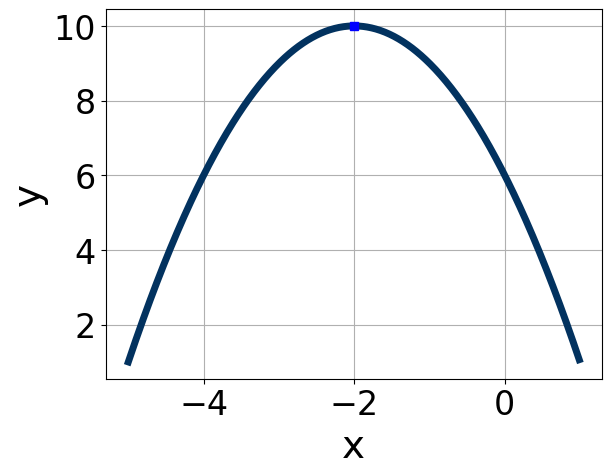
\includegraphics[width=0.5\textwidth]{../Figures/quadraticGraphToEquationA.png}
\end{center}
\begin{enumerate}[label=\Alph*.]
\item \( a \in [-2, -0.8], \hspace*{5mm} b \in [1, 6], \text{ and } \hspace*{5mm} c \in [-14, -10] \)
\item \( a \in [-2, -0.8], \hspace*{5mm} b \in [-5, -3], \text{ and } \hspace*{5mm} c \in [5, 9] \)
\item \( a \in [-2, -0.8], \hspace*{5mm} b \in [1, 6], \text{ and } \hspace*{5mm} c \in [5, 9] \)
\item \( a \in [-0.3, 1.8], \hspace*{5mm} b \in [-5, -3], \text{ and } \hspace*{5mm} c \in [11, 15] \)
\item \( a \in [-0.3, 1.8], \hspace*{5mm} b \in [1, 6], \text{ and } \hspace*{5mm} c \in [11, 15] \)

\end{enumerate} }
\litem{
Factor the quadratic below. Then, choose the intervals that contain the constants in the form $(ax+b)(cx+d); b \leq d.$\[ 54x^{2} -57 x + 10 \]\begin{enumerate}[label=\Alph*.]
\item \( a \in [1.9, 3.1], \hspace*{5mm} b \in [-6, -1], \hspace*{5mm} c \in [25.3, 27.05], \text{ and } \hspace*{5mm} d \in [-7, 4] \)
\item \( a \in [4.5, 6.5], \hspace*{5mm} b \in [-6, -1], \hspace*{5mm} c \in [7.67, 10.95], \text{ and } \hspace*{5mm} d \in [-7, 4] \)
\item \( a \in [0.8, 1.2], \hspace*{5mm} b \in [-48, -41], \hspace*{5mm} c \in [0.42, 1.12], \text{ and } \hspace*{5mm} d \in [-18, -8] \)
\item \( a \in [16.8, 19.6], \hspace*{5mm} b \in [-6, -1], \hspace*{5mm} c \in [2.05, 3.54], \text{ and } \hspace*{5mm} d \in [-7, 4] \)
\item \( \text{None of the above.} \)

\end{enumerate} }
\litem{
Solve the quadratic equation below. Then, choose the intervals that the solutions $x_1$ and $x_2$ belong to, with $x_1 \leq x_2$.\[ 10x^{2} -53 x + 36 = 0 \]\begin{enumerate}[label=\Alph*.]
\item \( x_1 \in [0.18, 0.29] \text{ and } x_2 \in [12.91, 13.59] \)
\item \( x_1 \in [0.58, 0.86] \text{ and } x_2 \in [4.23, 4.93] \)
\item \( x_1 \in [7.8, 8.15] \text{ and } x_2 \in [44.43, 45.75] \)
\item \( x_1 \in [0.85, 1.09] \text{ and } x_2 \in [3.99, 4.38] \)
\item \( x_1 \in [1.49, 1.94] \text{ and } x_2 \in [2.18, 2.4] \)

\end{enumerate} }
\litem{
Write the equation of the graph presented below in the form $f(x)=ax^2+bx+c$, assuming  $a=1$ or $a=-1$. Then, choose the intervals that $a, b,$ and $c$ belong to.
\begin{center}
    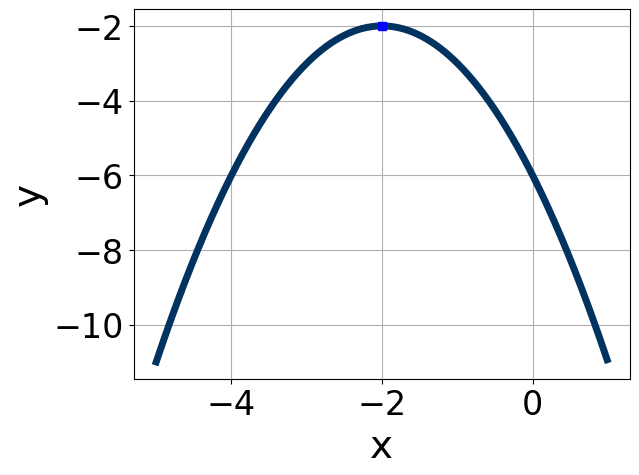
\includegraphics[width=0.5\textwidth]{../Figures/quadraticGraphToEquationCopyA.png}
\end{center}
\begin{enumerate}[label=\Alph*.]
\item \( a \in [-1.8, -0.5], \hspace*{5mm} b \in [4, 5], \text{ and } \hspace*{5mm} c \in [-4, -1] \)
\item \( a \in [0.6, 2.4], \hspace*{5mm} b \in [4, 5], \text{ and } \hspace*{5mm} c \in [-1, 3] \)
\item \( a \in [0.6, 2.4], \hspace*{5mm} b \in [-7, 1], \text{ and } \hspace*{5mm} c \in [-1, 3] \)
\item \( a \in [-1.8, -0.5], \hspace*{5mm} b \in [4, 5], \text{ and } \hspace*{5mm} c \in [-6, -4] \)
\item \( a \in [-1.8, -0.5], \hspace*{5mm} b \in [-7, 1], \text{ and } \hspace*{5mm} c \in [-6, -4] \)

\end{enumerate} }
\litem{
Solve the quadratic equation below. Then, choose the intervals that the solutions belong to, with $x_1 \leq x_2$ (if they exist).\[ 19x^{2} -13 x -8 = 0 \]\begin{enumerate}[label=\Alph*.]
\item \( x_1 \in [-1.16, -1] \text{ and } x_2 \in [0.32, 0.93] \)
\item \( x_1 \in [-0.86, 0.52] \text{ and } x_2 \in [0.53, 1.65] \)
\item \( x_1 \in [-8.02, -7.19] \text{ and } x_2 \in [20.31, 20.63] \)
\item \( x_1 \in [-27.65, -26.74] \text{ and } x_2 \in [27.96, 28.45] \)
\item \( \text{There are no Real solutions.} \)

\end{enumerate} }
\litem{
Factor the quadratic below. Then, choose the intervals that contain the constants in the form $(ax+b)(cx+d); b \leq d.$\[ 36x^{2} +60 x + 25 \]\begin{enumerate}[label=\Alph*.]
\item \( a \in [1.41, 3.78], \hspace*{5mm} b \in [5, 9], \hspace*{5mm} c \in [10.94, 13.08], \text{ and } \hspace*{5mm} d \in [4, 14] \)
\item \( a \in [17.03, 18.26], \hspace*{5mm} b \in [5, 9], \hspace*{5mm} c \in [1.93, 2.21], \text{ and } \hspace*{5mm} d \in [4, 14] \)
\item \( a \in [4.42, 6.01], \hspace*{5mm} b \in [5, 9], \hspace*{5mm} c \in [5.68, 7.39], \text{ and } \hspace*{5mm} d \in [4, 14] \)
\item \( a \in [0.67, 1.6], \hspace*{5mm} b \in [26, 37], \hspace*{5mm} c \in [0.92, 1.75], \text{ and } \hspace*{5mm} d \in [29, 31] \)
\item \( \text{None of the above.} \)

\end{enumerate} }
\litem{
Graph the equation below.\[ f(x) = -(x+1)^2 - 15 \]\begin{enumerate}[label=\Alph*.]
\begin{multicols}{2}\item 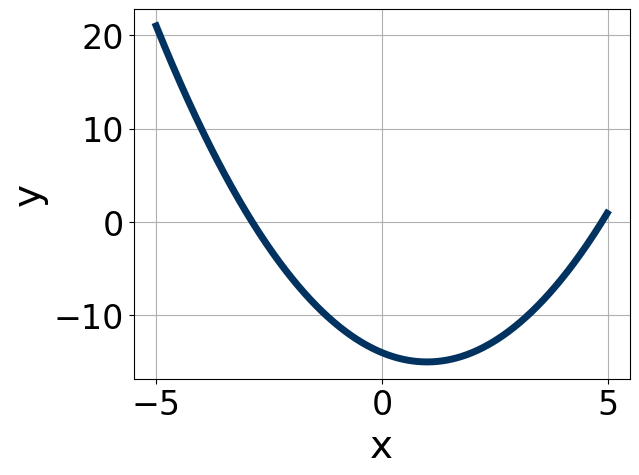
\includegraphics[width = 0.3\textwidth]{../Figures/quadraticEquationToGraphAA.png}\item 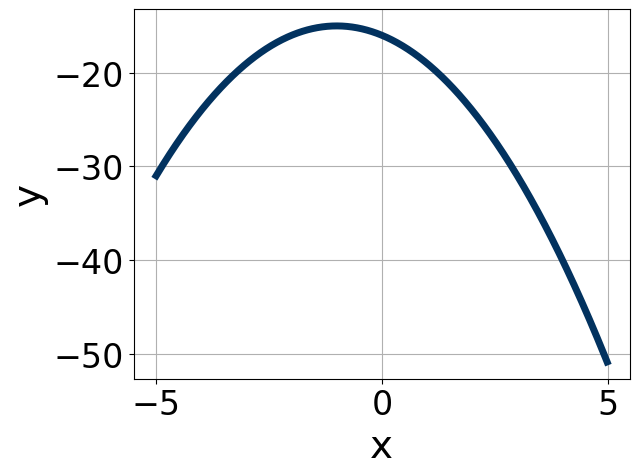
\includegraphics[width = 0.3\textwidth]{../Figures/quadraticEquationToGraphBA.png}\item 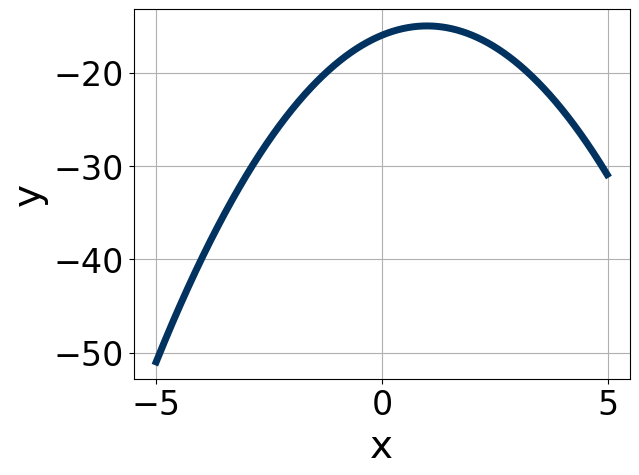
\includegraphics[width = 0.3\textwidth]{../Figures/quadraticEquationToGraphCA.png}\item 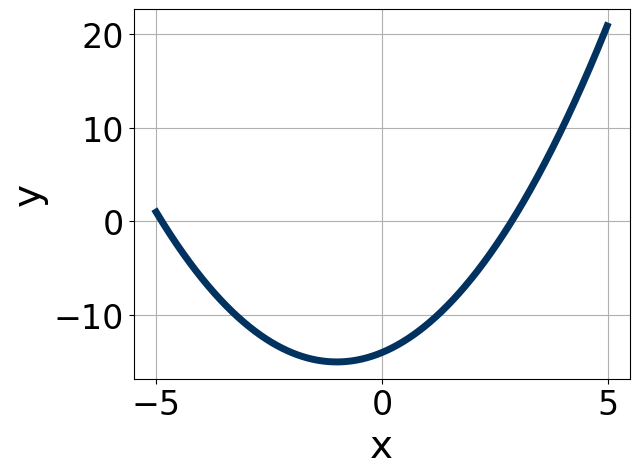
\includegraphics[width = 0.3\textwidth]{../Figures/quadraticEquationToGraphDA.png}\end{multicols}\item None of the above.
\end{enumerate} }
\litem{
Solve the quadratic equation below. Then, choose the intervals that the solutions belong to, with $x_1 \leq x_2$ (if they exist).\[ 10x^{2} +12 x -5 = 0 \]\begin{enumerate}[label=\Alph*.]
\item \( x_1 \in [-20.1, -17.9] \text{ and } x_2 \in [16.1, 18.4] \)
\item \( x_1 \in [-0.5, 1.9] \text{ and } x_2 \in [1.5, 2.7] \)
\item \( x_1 \in [-17.2, -15.1] \text{ and } x_2 \in [2.7, 5.6] \)
\item \( x_1 \in [-1.9, -0.4] \text{ and } x_2 \in [-0.6, 0.7] \)
\item \( \text{There are no Real solutions.} \)

\end{enumerate} }
\litem{
Solve the quadratic equation below. Then, choose the intervals that the solutions $x_1$ and $x_2$ belong to, with $x_1 \leq x_2$.\[ 15x^{2} +8 x -16 = 0 \]\begin{enumerate}[label=\Alph*.]
\item \( x_1 \in [-1.78, -0.94] \text{ and } x_2 \in [0.7, 1.03] \)
\item \( x_1 \in [-4.45, -3.43] \text{ and } x_2 \in [0.25, 0.36] \)
\item \( x_1 \in [-0.71, 0.61] \text{ and } x_2 \in [1.41, 1.67] \)
\item \( x_1 \in [-20.84, -18.76] \text{ and } x_2 \in [11.92, 12.11] \)
\item \( x_1 \in [-2.91, -1.6] \text{ and } x_2 \in [0.36, 0.47] \)

\end{enumerate} }
\litem{
Graph the equation below.\[ f(x) = (x+2)^2 - 15 \]\begin{enumerate}[label=\Alph*.]
\begin{multicols}{2}\item 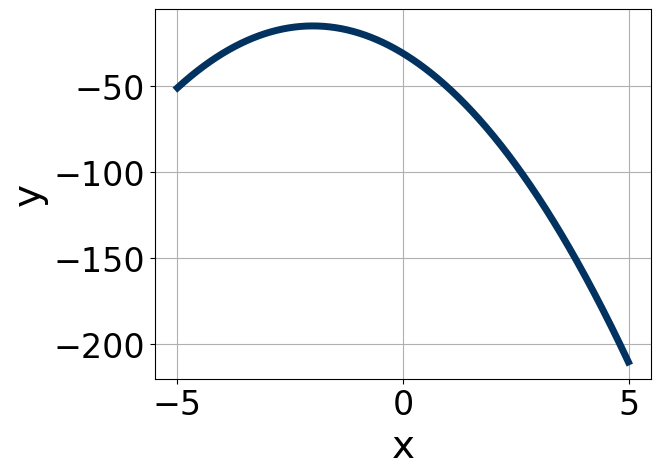
\includegraphics[width = 0.3\textwidth]{../Figures/quadraticEquationToGraphCopyAA.png}\item 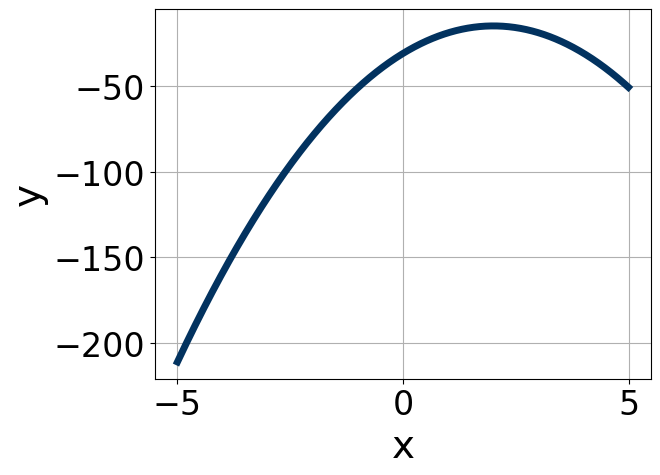
\includegraphics[width = 0.3\textwidth]{../Figures/quadraticEquationToGraphCopyBA.png}\item 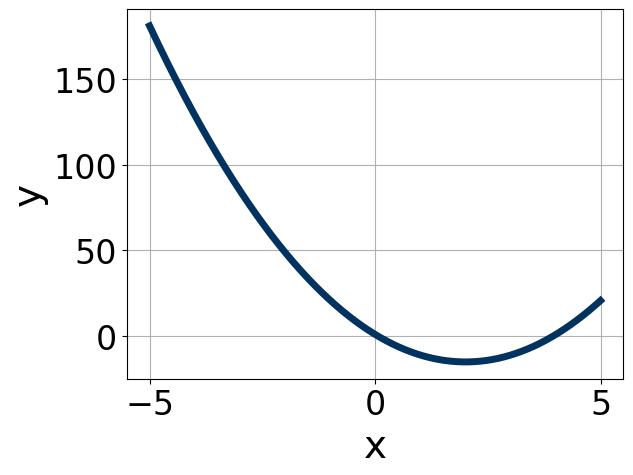
\includegraphics[width = 0.3\textwidth]{../Figures/quadraticEquationToGraphCopyCA.png}\item 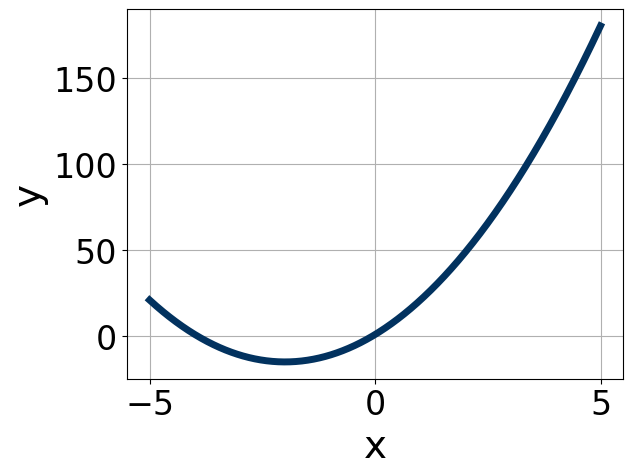
\includegraphics[width = 0.3\textwidth]{../Figures/quadraticEquationToGraphCopyDA.png}\end{multicols}\item None of the above.
\end{enumerate} }
\litem{
Write the equation of the graph presented below in the form $f(x)=ax^2+bx+c$, assuming  $a=1$ or $a=-1$. Then, choose the intervals that $a, b,$ and $c$ belong to.
\begin{center}
    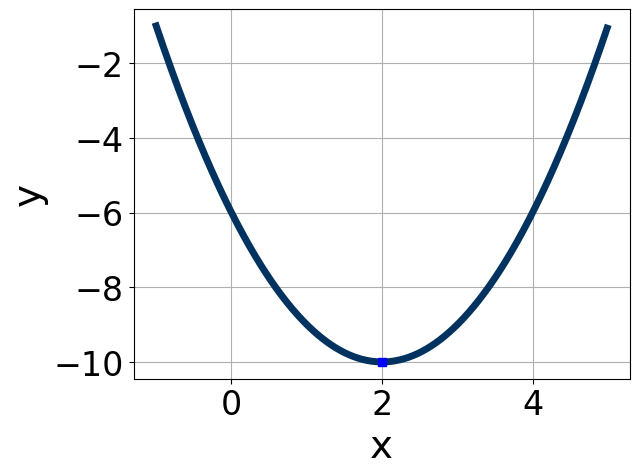
\includegraphics[width=0.5\textwidth]{../Figures/quadraticGraphToEquationB.png}
\end{center}
\begin{enumerate}[label=\Alph*.]
\item \( a \in [-4, 0], \hspace*{5mm} b \in [0, 7], \text{ and } \hspace*{5mm} c \in [-15, -12] \)
\item \( a \in [0, 2], \hspace*{5mm} b \in [-4, -2], \text{ and } \hspace*{5mm} c \in [-8, -4] \)
\item \( a \in [0, 2], \hspace*{5mm} b \in [0, 7], \text{ and } \hspace*{5mm} c \in [14, 17] \)
\item \( a \in [-4, 0], \hspace*{5mm} b \in [-4, -2], \text{ and } \hspace*{5mm} c \in [-15, -12] \)
\item \( a \in [0, 2], \hspace*{5mm} b \in [0, 7], \text{ and } \hspace*{5mm} c \in [-8, -4] \)

\end{enumerate} }
\litem{
Factor the quadratic below. Then, choose the intervals that contain the constants in the form $(ax+b)(cx+d); b \leq d.$\[ 24x^{2} +38 x + 15 \]\begin{enumerate}[label=\Alph*.]
\item \( a \in [-1.31, 1.93], \hspace*{5mm} b \in [13, 22], \hspace*{5mm} c \in [-0.16, 1.34], \text{ and } \hspace*{5mm} d \in [19, 24] \)
\item \( a \in [3.29, 4.95], \hspace*{5mm} b \in [-3, 6], \hspace*{5mm} c \in [5.47, 7.45], \text{ and } \hspace*{5mm} d \in [4, 12] \)
\item \( a \in [6.96, 9.03], \hspace*{5mm} b \in [-3, 6], \hspace*{5mm} c \in [2.25, 4.92], \text{ and } \hspace*{5mm} d \in [4, 12] \)
\item \( a \in [1.81, 2.88], \hspace*{5mm} b \in [-3, 6], \hspace*{5mm} c \in [10.17, 12.99], \text{ and } \hspace*{5mm} d \in [4, 12] \)
\item \( \text{None of the above.} \)

\end{enumerate} }
\litem{
Solve the quadratic equation below. Then, choose the intervals that the solutions $x_1$ and $x_2$ belong to, with $x_1 \leq x_2$.\[ 15x^{2} +38 x + 24 = 0 \]\begin{enumerate}[label=\Alph*.]
\item \( x_1 \in [-1.77, -0.84] \text{ and } x_2 \in [-1.32, -1.11] \)
\item \( x_1 \in [-2.5, -2] \text{ and } x_2 \in [-0.68, -0.61] \)
\item \( x_1 \in [-6.32, -5.86] \text{ and } x_2 \in [-0.46, -0.16] \)
\item \( x_1 \in [-20.14, -19.4] \text{ and } x_2 \in [-18.02, -17.99] \)
\item \( x_1 \in [-2.75, -2.44] \text{ and } x_2 \in [-0.62, -0.44] \)

\end{enumerate} }
\litem{
Write the equation of the graph presented below in the form $f(x)=ax^2+bx+c$, assuming  $a=1$ or $a=-1$. Then, choose the intervals that $a, b,$ and $c$ belong to.
\begin{center}
    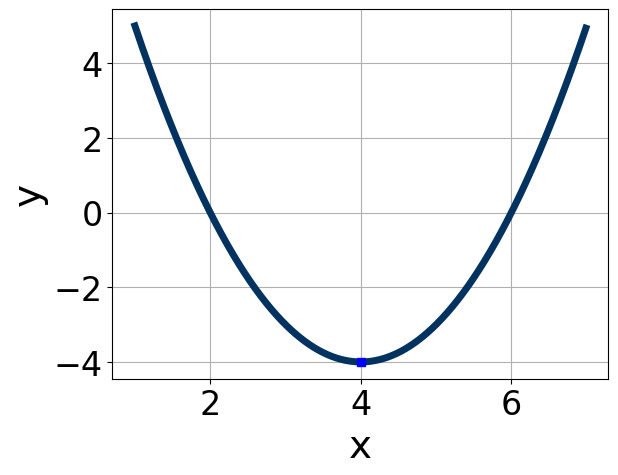
\includegraphics[width=0.5\textwidth]{../Figures/quadraticGraphToEquationCopyB.png}
\end{center}
\begin{enumerate}[label=\Alph*.]
\item \( a \in [0, 2], \hspace*{5mm} b \in [8, 9], \text{ and } \hspace*{5mm} c \in [12, 15] \)
\item \( a \in [0, 2], \hspace*{5mm} b \in [-12, -5], \text{ and } \hspace*{5mm} c \in [12, 15] \)
\item \( a \in [-2, 0], \hspace*{5mm} b \in [-12, -5], \text{ and } \hspace*{5mm} c \in [-22, -18] \)
\item \( a \in [0, 2], \hspace*{5mm} b \in [8, 9], \text{ and } \hspace*{5mm} c \in [20, 22] \)
\item \( a \in [-2, 0], \hspace*{5mm} b \in [8, 9], \text{ and } \hspace*{5mm} c \in [-22, -18] \)

\end{enumerate} }
\litem{
Solve the quadratic equation below. Then, choose the intervals that the solutions belong to, with $x_1 \leq x_2$ (if they exist).\[ 20x^{2} -7 x -2 = 0 \]\begin{enumerate}[label=\Alph*.]
\item \( x_1 \in [-0.96, -0.33] \text{ and } x_2 \in [0, 0.5] \)
\item \( x_1 \in [-0.37, -0.04] \text{ and } x_2 \in [0.2, 1.1] \)
\item \( x_1 \in [-3.87, -3.4] \text{ and } x_2 \in [8.8, 11.1] \)
\item \( x_1 \in [-14.29, -14.01] \text{ and } x_2 \in [12.9, 15.8] \)
\item \( \text{There are no Real solutions.} \)

\end{enumerate} }
\litem{
Factor the quadratic below. Then, choose the intervals that contain the constants in the form $(ax+b)(cx+d); b \leq d.$\[ 36x^{2} -60 x + 25 \]\begin{enumerate}[label=\Alph*.]
\item \( a \in [11.1, 12.9], \hspace*{5mm} b \in [-7, -4], \hspace*{5mm} c \in [1.5, 3.3], \text{ and } \hspace*{5mm} d \in [-7, -3] \)
\item \( a \in [-1.7, 2.2], \hspace*{5mm} b \in [-32, -26], \hspace*{5mm} c \in [-1.2, 2.6], \text{ and } \hspace*{5mm} d \in [-31, -27] \)
\item \( a \in [5.9, 7.2], \hspace*{5mm} b \in [-7, -4], \hspace*{5mm} c \in [5.4, 9.9], \text{ and } \hspace*{5mm} d \in [-7, -3] \)
\item \( a \in [2.4, 4.1], \hspace*{5mm} b \in [-7, -4], \hspace*{5mm} c \in [11.9, 15.7], \text{ and } \hspace*{5mm} d \in [-7, -3] \)
\item \( \text{None of the above.} \)

\end{enumerate} }
\litem{
Graph the equation below.\[ f(x) = -(x+1)^2 - 12 \]\begin{enumerate}[label=\Alph*.]
\begin{multicols}{2}\item 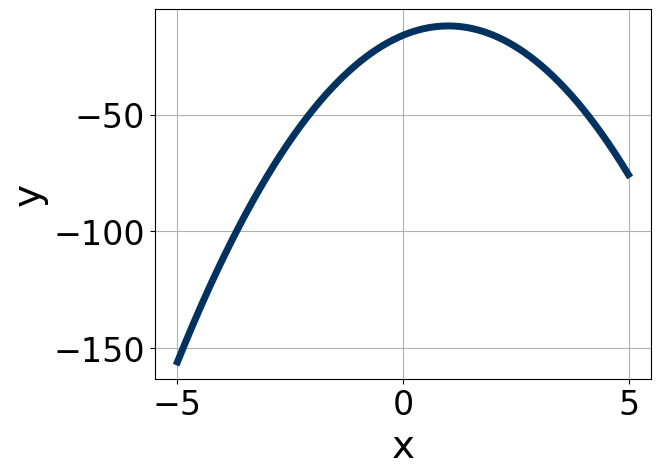
\includegraphics[width = 0.3\textwidth]{../Figures/quadraticEquationToGraphAB.png}\item 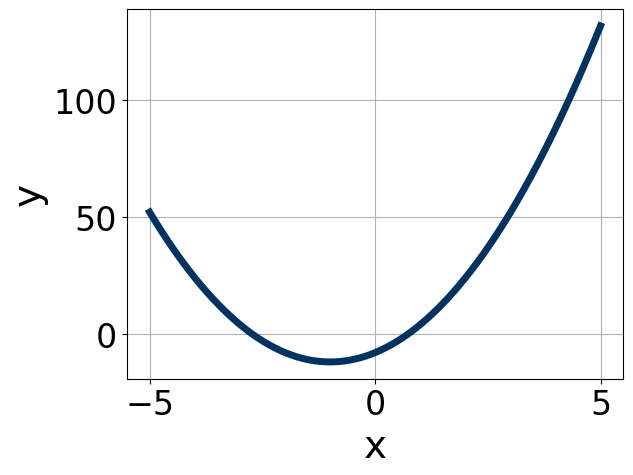
\includegraphics[width = 0.3\textwidth]{../Figures/quadraticEquationToGraphBB.png}\item 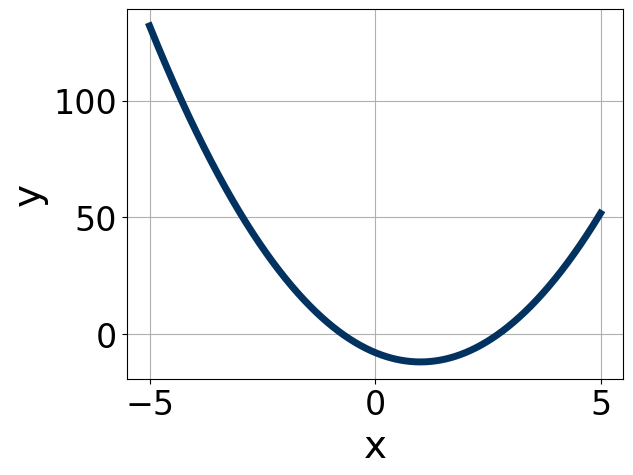
\includegraphics[width = 0.3\textwidth]{../Figures/quadraticEquationToGraphCB.png}\item 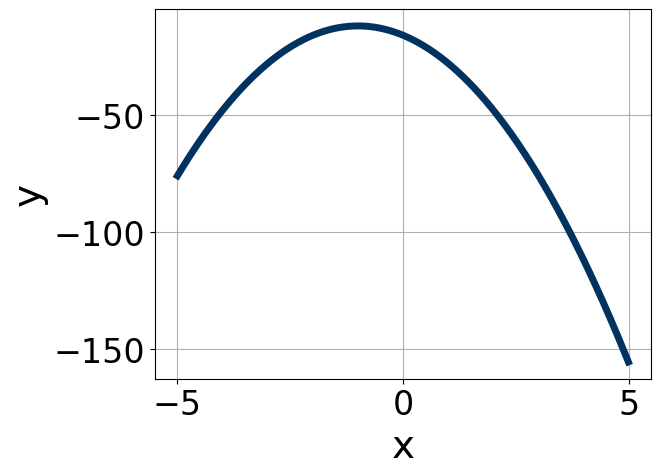
\includegraphics[width = 0.3\textwidth]{../Figures/quadraticEquationToGraphDB.png}\end{multicols}\item None of the above.
\end{enumerate} }
\litem{
Solve the quadratic equation below. Then, choose the intervals that the solutions belong to, with $x_1 \leq x_2$ (if they exist).\[ 14x^{2} -11 x -7 = 0 \]\begin{enumerate}[label=\Alph*.]
\item \( x_1 \in [-2.5, -0.9] \text{ and } x_2 \in [-1.1, 0.9] \)
\item \( x_1 \in [-5.9, -4.1] \text{ and } x_2 \in [15.9, 17.2] \)
\item \( x_1 \in [-22.7, -21.6] \text{ and } x_2 \in [22.9, 25.3] \)
\item \( x_1 \in [-1.2, 1.4] \text{ and } x_2 \in [1, 2.7] \)
\item \( \text{There are no Real solutions.} \)

\end{enumerate} }
\litem{
Solve the quadratic equation below. Then, choose the intervals that the solutions $x_1$ and $x_2$ belong to, with $x_1 \leq x_2$.\[ 15x^{2} -2 x -24 = 0 \]\begin{enumerate}[label=\Alph*.]
\item \( x_1 \in [-6.19, -5.18] \text{ and } x_2 \in [0.25, 0.47] \)
\item \( x_1 \in [-0.78, -0.32] \text{ and } x_2 \in [2.24, 2.79] \)
\item \( x_1 \in [-1.35, -0.62] \text{ and } x_2 \in [0.91, 1.51] \)
\item \( x_1 \in [-2.54, -2.24] \text{ and } x_2 \in [0.48, 0.82] \)
\item \( x_1 \in [-18.5, -17.74] \text{ and } x_2 \in [19.91, 20.15] \)

\end{enumerate} }
\litem{
Graph the equation below.\[ f(x) = -(x+1)^2 - 14 \]\begin{enumerate}[label=\Alph*.]
\begin{multicols}{2}\item 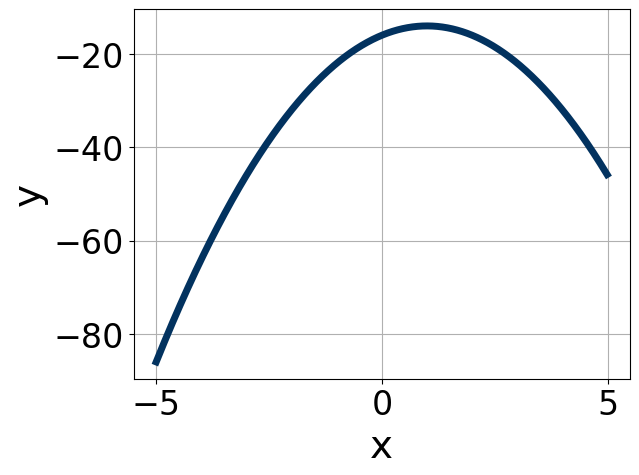
\includegraphics[width = 0.3\textwidth]{../Figures/quadraticEquationToGraphCopyAB.png}\item 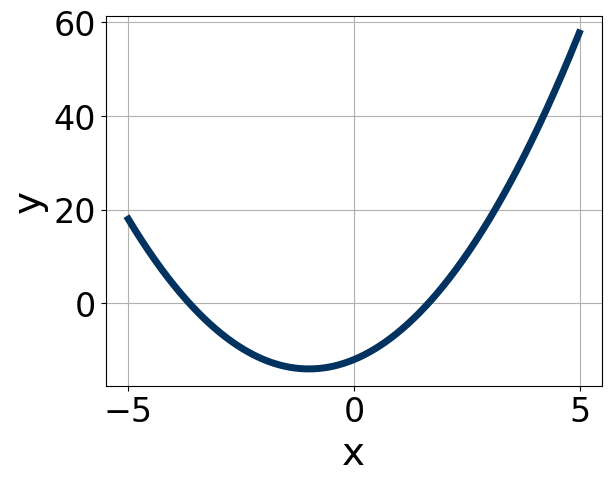
\includegraphics[width = 0.3\textwidth]{../Figures/quadraticEquationToGraphCopyBB.png}\item 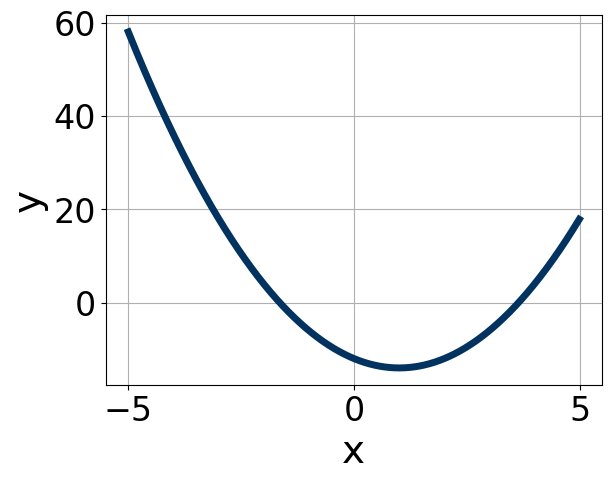
\includegraphics[width = 0.3\textwidth]{../Figures/quadraticEquationToGraphCopyCB.png}\item 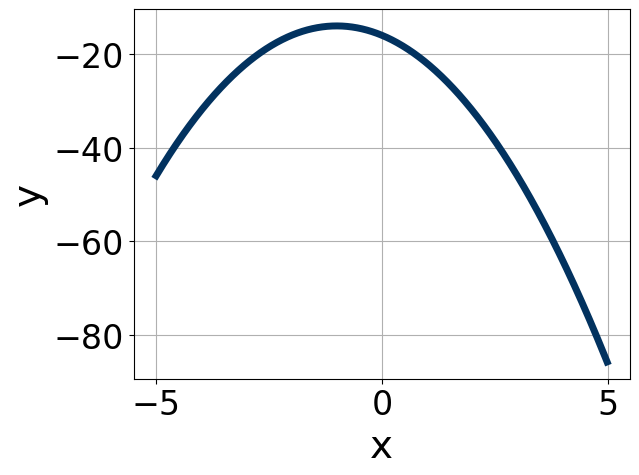
\includegraphics[width = 0.3\textwidth]{../Figures/quadraticEquationToGraphCopyDB.png}\end{multicols}\item None of the above.
\end{enumerate} }
\litem{
Write the equation of the graph presented below in the form $f(x)=ax^2+bx+c$, assuming  $a=1$ or $a=-1$. Then, choose the intervals that $a, b,$ and $c$ belong to.
\begin{center}
    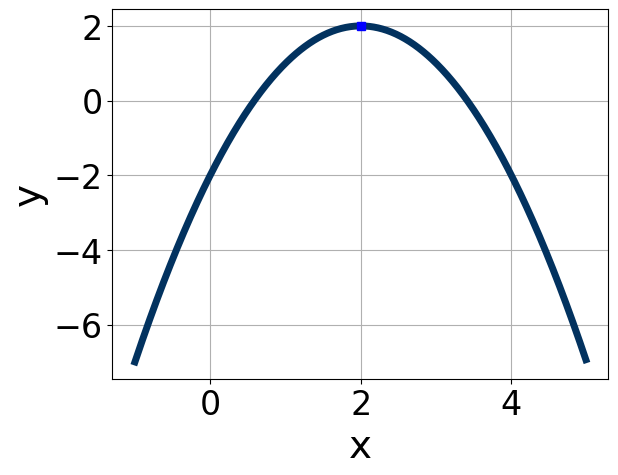
\includegraphics[width=0.5\textwidth]{../Figures/quadraticGraphToEquationC.png}
\end{center}
\begin{enumerate}[label=\Alph*.]
\item \( a \in [-1, 0], \hspace*{5mm} b \in [-6, -3], \text{ and } \hspace*{5mm} c \in [-4.1, -1.3] \)
\item \( a \in [-1, 0], \hspace*{5mm} b \in [3, 8], \text{ and } \hspace*{5mm} c \in [-4.1, -1.3] \)
\item \( a \in [-1, 0], \hspace*{5mm} b \in [-6, -3], \text{ and } \hspace*{5mm} c \in [-6.8, -4.6] \)
\item \( a \in [0, 3], \hspace*{5mm} b \in [3, 8], \text{ and } \hspace*{5mm} c \in [5.3, 6.8] \)
\item \( a \in [0, 3], \hspace*{5mm} b \in [-6, -3], \text{ and } \hspace*{5mm} c \in [5.3, 6.8] \)

\end{enumerate} }
\litem{
Factor the quadratic below. Then, choose the intervals that contain the constants in the form $(ax+b)(cx+d); b \leq d.$\[ 81x^{2} -27 x -10 \]\begin{enumerate}[label=\Alph*.]
\item \( a \in [26.84, 27.15], \hspace*{5mm} b \in [-8, -1], \hspace*{5mm} c \in [1.2, 3.4], \text{ and } \hspace*{5mm} d \in [1, 4] \)
\item \( a \in [8.76, 9.27], \hspace*{5mm} b \in [-8, -1], \hspace*{5mm} c \in [6.6, 13.6], \text{ and } \hspace*{5mm} d \in [1, 4] \)
\item \( a \in [0.38, 1.02], \hspace*{5mm} b \in [-48, -39], \hspace*{5mm} c \in [0.8, 1.4], \text{ and } \hspace*{5mm} d \in [18, 23] \)
\item \( a \in [1.84, 3.62], \hspace*{5mm} b \in [-8, -1], \hspace*{5mm} c \in [24.7, 28], \text{ and } \hspace*{5mm} d \in [1, 4] \)
\item \( \text{None of the above.} \)

\end{enumerate} }
\litem{
Solve the quadratic equation below. Then, choose the intervals that the solutions $x_1$ and $x_2$ belong to, with $x_1 \leq x_2$.\[ 10x^{2} +33 x -54 = 0 \]\begin{enumerate}[label=\Alph*.]
\item \( x_1 \in [-13.5, -12.5] \text{ and } x_2 \in [0.11, 0.52] \)
\item \( x_1 \in [-6.5, -3.5] \text{ and } x_2 \in [1.14, 1.33] \)
\item \( x_1 \in [-1.5, 4.5] \text{ and } x_2 \in [3.34, 3.77] \)
\item \( x_1 \in [-13, -8] \text{ and } x_2 \in [0.49, 0.76] \)
\item \( x_1 \in [-46, -44] \text{ and } x_2 \in [11.7, 12.23] \)

\end{enumerate} }
\litem{
Write the equation of the graph presented below in the form $f(x)=ax^2+bx+c$, assuming  $a=1$ or $a=-1$. Then, choose the intervals that $a, b,$ and $c$ belong to.
\begin{center}
    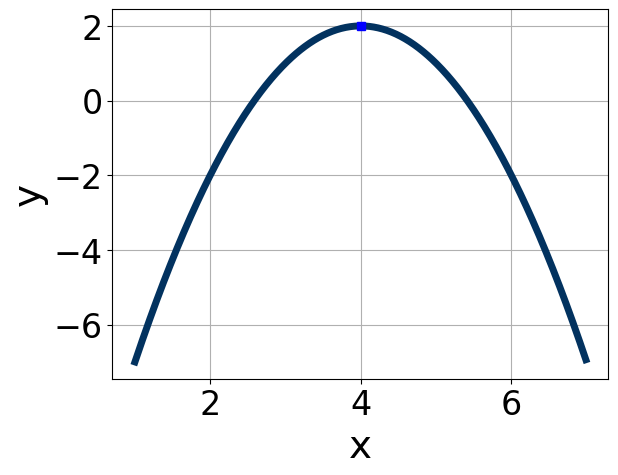
\includegraphics[width=0.5\textwidth]{../Figures/quadraticGraphToEquationCopyC.png}
\end{center}
\begin{enumerate}[label=\Alph*.]
\item \( a \in [0, 5], \hspace*{5mm} b \in [-11, -7], \text{ and } \hspace*{5mm} c \in [17, 20] \)
\item \( a \in [-6, 0], \hspace*{5mm} b \in [8, 10], \text{ and } \hspace*{5mm} c \in [-14, -12] \)
\item \( a \in [-6, 0], \hspace*{5mm} b \in [-11, -7], \text{ and } \hspace*{5mm} c \in [-18, -16] \)
\item \( a \in [0, 5], \hspace*{5mm} b \in [8, 10], \text{ and } \hspace*{5mm} c \in [17, 20] \)
\item \( a \in [-6, 0], \hspace*{5mm} b \in [-11, -7], \text{ and } \hspace*{5mm} c \in [-14, -12] \)

\end{enumerate} }
\litem{
Solve the quadratic equation below. Then, choose the intervals that the solutions belong to, with $x_1 \leq x_2$ (if they exist).\[ -20x^{2} -13 x + 3 = 0 \]\begin{enumerate}[label=\Alph*.]
\item \( x_1 \in [-1.46, -0.41] \text{ and } x_2 \in [-0.43, 0.72] \)
\item \( x_1 \in [-4.25, -3.01] \text{ and } x_2 \in [15.81, 16.8] \)
\item \( x_1 \in [-21.08, -20.1] \text{ and } x_2 \in [18.98, 20.41] \)
\item \( x_1 \in [-0.59, -0.06] \text{ and } x_2 \in [0.27, 1.63] \)
\item \( \text{There are no Real solutions.} \)

\end{enumerate} }
\litem{
Factor the quadratic below. Then, choose the intervals that contain the constants in the form $(ax+b)(cx+d); b \leq d.$\[ 36x^{2} -60 x + 25 \]\begin{enumerate}[label=\Alph*.]
\item \( a \in [4.75, 6.2], \hspace*{5mm} b \in [-8, -4], \hspace*{5mm} c \in [5.94, 6.09], \text{ and } \hspace*{5mm} d \in [-7, -3] \)
\item \( a \in [0.76, 1.49], \hspace*{5mm} b \in [-34, -25], \hspace*{5mm} c \in [0.54, 1.72], \text{ and } \hspace*{5mm} d \in [-33, -26] \)
\item \( a \in [1.42, 2.16], \hspace*{5mm} b \in [-8, -4], \hspace*{5mm} c \in [17.56, 18.04], \text{ and } \hspace*{5mm} d \in [-7, -3] \)
\item \( a \in [17.82, 18.42], \hspace*{5mm} b \in [-8, -4], \hspace*{5mm} c \in [1.88, 2.43], \text{ and } \hspace*{5mm} d \in [-7, -3] \)
\item \( \text{None of the above.} \)

\end{enumerate} }
\litem{
Graph the equation below.\[ f(x) = -(x-2)^2 + 18 \]\begin{enumerate}[label=\Alph*.]
\begin{multicols}{2}\item 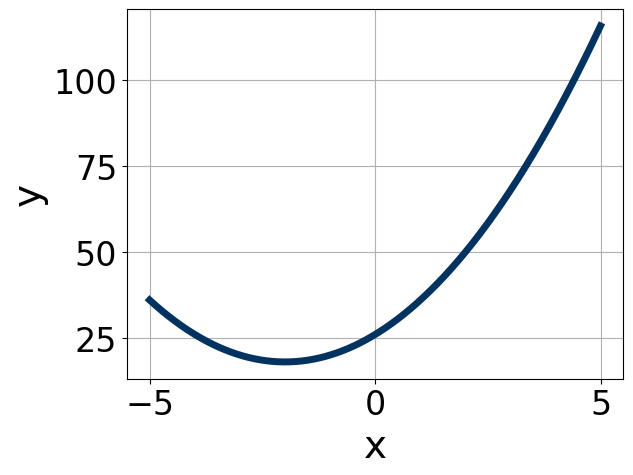
\includegraphics[width = 0.3\textwidth]{../Figures/quadraticEquationToGraphAC.png}\item 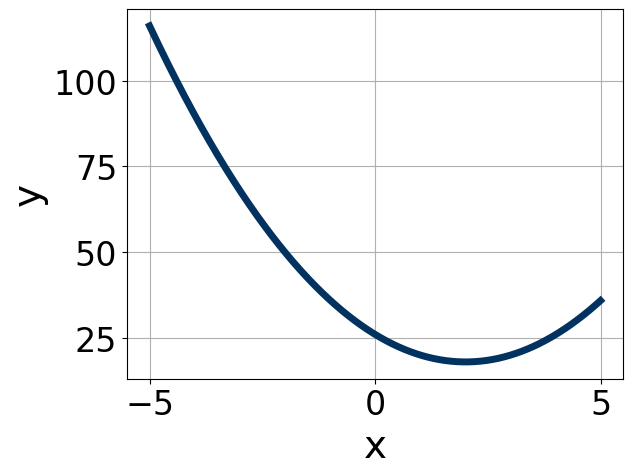
\includegraphics[width = 0.3\textwidth]{../Figures/quadraticEquationToGraphBC.png}\item 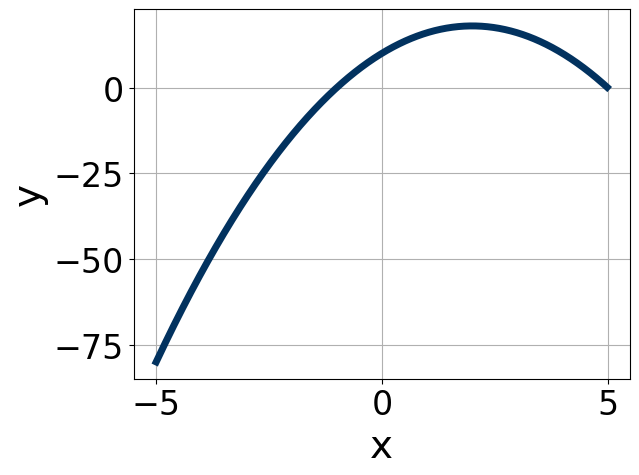
\includegraphics[width = 0.3\textwidth]{../Figures/quadraticEquationToGraphCC.png}\item 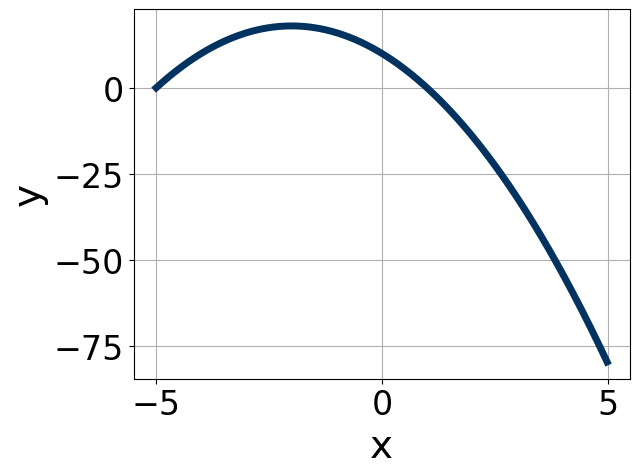
\includegraphics[width = 0.3\textwidth]{../Figures/quadraticEquationToGraphDC.png}\end{multicols}\item None of the above.
\end{enumerate} }
\litem{
Solve the quadratic equation below. Then, choose the intervals that the solutions belong to, with $x_1 \leq x_2$ (if they exist).\[ 15x^{2} +8 x -5 = 0 \]\begin{enumerate}[label=\Alph*.]
\item \( x_1 \in [-1.09, -0.48] \text{ and } x_2 \in [0.05, 0.52] \)
\item \( x_1 \in [-0.82, -0.3] \text{ and } x_2 \in [0.86, 1.21] \)
\item \( x_1 \in [-20.11, -18.33] \text{ and } x_2 \in [18.23, 19.14] \)
\item \( x_1 \in [-14.16, -13.12] \text{ and } x_2 \in [5.25, 5.92] \)
\item \( \text{There are no Real solutions.} \)

\end{enumerate} }
\litem{
Solve the quadratic equation below. Then, choose the intervals that the solutions $x_1$ and $x_2$ belong to, with $x_1 \leq x_2$.\[ 10x^{2} +57 x + 54 = 0 \]\begin{enumerate}[label=\Alph*.]
\item \( x_1 \in [-9.26, -8.66] \text{ and } x_2 \in [-0.62, -0.53] \)
\item \( x_1 \in [-4.2, -3.05] \text{ and } x_2 \in [-1.52, -1.39] \)
\item \( x_1 \in [-14.3, -13.15] \text{ and } x_2 \in [-0.49, -0.39] \)
\item \( x_1 \in [-4.83, -3.98] \text{ and } x_2 \in [-1.44, -1.11] \)
\item \( x_1 \in [-45.02, -44.91] \text{ and } x_2 \in [-12.01, -11.94] \)

\end{enumerate} }
\litem{
Graph the equation below.\[ f(x) = -(x+4)^2 + 16 \]\begin{enumerate}[label=\Alph*.]
\begin{multicols}{2}\item 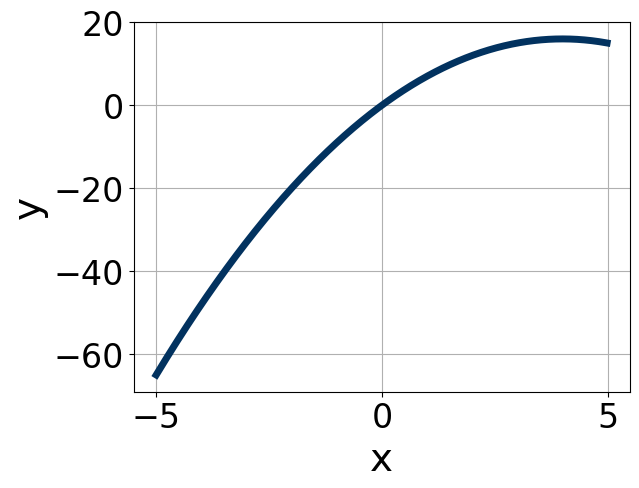
\includegraphics[width = 0.3\textwidth]{../Figures/quadraticEquationToGraphCopyAC.png}\item 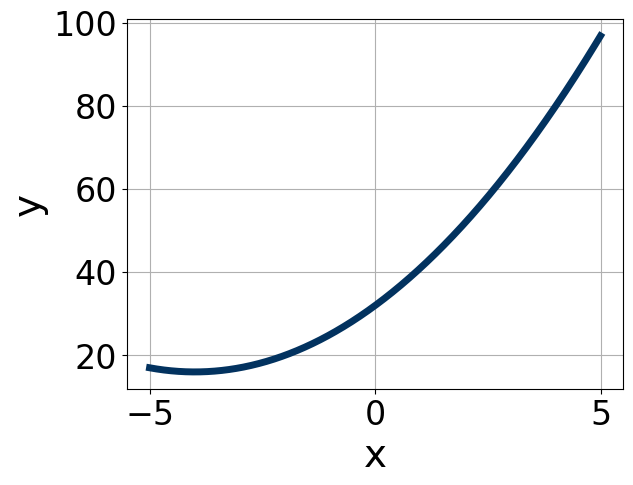
\includegraphics[width = 0.3\textwidth]{../Figures/quadraticEquationToGraphCopyBC.png}\item 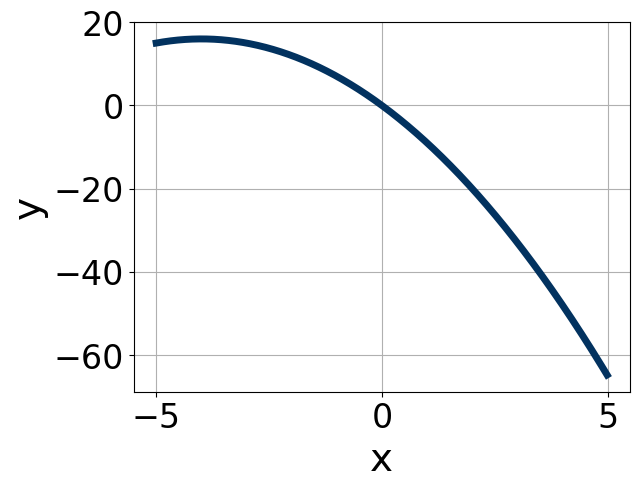
\includegraphics[width = 0.3\textwidth]{../Figures/quadraticEquationToGraphCopyCC.png}\item 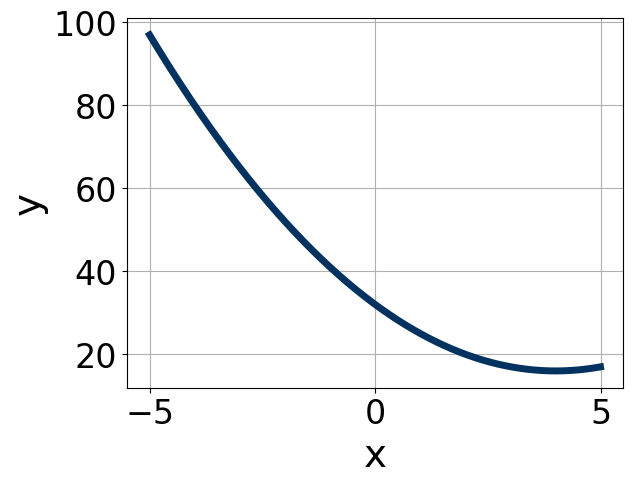
\includegraphics[width = 0.3\textwidth]{../Figures/quadraticEquationToGraphCopyDC.png}\end{multicols}\item None of the above.
\end{enumerate} }
\end{enumerate}

\end{document}